%==============================================================================
% tento soubor pouzijte jako zaklad
% this file should be used as a base for the thesis
% (c) 2008 Michal Bidlo
% E-mail: bidlom AT fit vutbr cz
% Šablonu upravil / template edited by: Ing. Jaroslav Dytrych, dytrych@fit.vutbr.cz
%==============================================================================
% kodovaní: UTF-8 (zmena prikazem iconv, recode nebo cstocs)
% encoding: UTF-8 (you can change it by command iconv, recode or cstocs)
%------------------------------------------------------------------------------
% zpracování / processing: make, make pdf, make clean
%==============================================================================
% Soubory, které je nutné upravit: / Files which have to be edited:
%   projekt-20-literatura-bibliography.bib - literatura / bibliography
%   projekt-01-kapitoly-chapters.tex - obsah práce / the thesis content
%   projekt-30-prilohy-appendices.tex - přílohy / appendices
%==============================================================================
\documentclass[english]{fitthesis} 

% bez zadání - pro začátek práce, aby nebyl problém s překladem
%\documentclass[english]{fitthesis} % without assignment - for the work start to avoid compilation problem
%\documentclass[zadani]{fitthesis} % odevzdani do wisu - odkazy jsou barevné
%\documentclass[english,zadani]{fitthesis} % for submission to the IS FIT - links are color
%\documentclass[zadani,print]{fitthesis} % pro tisk - odkazy jsou černé
%\documentclass[english,zadani,print]{fitthesis} % for the print - links are black
% * Je-li prace psana v anglickem jazyce, je zapotrebi u tridy pouzit 
%   parametr english nasledovne:
%   If thesis is written in english, it is necessary to use 
%   parameter english as follows:
%      \documentclass[english]{fitthesis}
% * Je-li prace psana ve slovenskem jazyce, je zapotrebi u tridy pouzit 
%   parametr slovak nasledovne:
%      \documentclass[slovak]{fitthesis}

% Základní balíčky jsou dole v souboru šablony fitthesis.cls
% Basic packages are at the bottom of template file fitthesis.cls
%zde muzeme vlozit vlastni balicky / you can place own packages here

%---rm---------------
\renewcommand{\rmdefault}{lmr}%zavede Latin Modern Roman jako rm / set Latin Modern Roman as rm
%---sf---------------
\renewcommand{\sfdefault}{qhv}%zavede TeX Gyre Heros jako sf
%---tt------------
\renewcommand{\ttdefault}{lmtt}% zavede Latin Modern tt jako tt

% vypne funkci šablony, která automaticky nahrazuje uvozovky,
% aby nebyly prováděny nevhodné náhrady v popisech API apod.
% disables function of the template which replaces quotation marks
% to avoid unnecessary replacements in the API descriptions etc.
\csdoublequotesoff

% =======================================================================
% balíček "hyperref" vytváří klikací odkazy v pdf, pokud tedy použijeme pdflatex
% problém je, že balíček hyperref musí být uveden jako poslední, takže nemůže
% být v šabloně
% "hyperref" package create clickable links in pdf if you are using pdflatex.
% Problem is that this package have to be introduced as the last one so it 
% can not be placed in the template file.
\ifWis
\ifx\pdfoutput\undefined % nejedeme pod pdflatexem / we are not using pdflatex
\else
  \usepackage{color}
  \usepackage[unicode,colorlinks,hyperindex,plainpages=false,pdftex]{hyperref}
  \definecolor{links}{rgb}{0.4,0.5,0}
  \definecolor{anchors}{rgb}{1,0,0}
  \def\AnchorColor{anchors}
  \def\LinkColor{links}
  \def\pdfBorderAttrs{/Border [0 0 0] }  % bez okrajů kolem odkazů / without margins around links
  \pdfcompresslevel=9
\fi
\else % pro tisk budou odkazy, na které se dá klikat, černé / for the print clickable links will be black
\ifx\pdfoutput\undefined % nejedeme pod pdflatexem / we are not using pdflatex
\else
  \usepackage{color}
  \usepackage[unicode,colorlinks,hyperindex,plainpages=false,pdftex,urlcolor=black,linkcolor=black,citecolor=black]{hyperref}
  \definecolor{links}{rgb}{0,0,0}
  \definecolor{anchors}{rgb}{0,0,0}
  \def\AnchorColor{anchors}
  \def\LinkColor{links}
  \def\pdfBorderAttrs{/Border [0 0 0] } % bez okrajů kolem odkazů / without margins around links
  \pdfcompresslevel=9
\fi
\fi
% Řešení problému, kdy klikací odkazy na obrázky vedou za obrázek
% This solves the problems with links which leads after the picture
\usepackage[all]{hypcap}
\usepackage{tikz}
\usepackage{url}
\usepackage{listings}

\hypersetup{
  colorlinks = true,
  linkcolor  = black
}

% Informace o práci/projektu / Information about the thesis
%---------------------------------------------------------------------------
\projectinfo{
  %Prace / Thesis
  project=SP,            %typ prace BP/SP/DP/DR  / thesis type (SP = term project)
  year=2017,             %rok odevzdání / year of submission
  date=\today,           %datum odevzdani / submission date
  %Nazev prace / thesis title
  title.cs={Abstrakce pro konečné automaty v analýze programů},  %nazev prace v cestine ci slovenstine (dle zadani) / thesis title in czech language (according to assignment)
  title.en={Abstraction for Finite Automata in Program \mbox{Analysis}}, %nazev prace v anglictine / thesis title in english
  %Autor / Author
  author={Dávid Bolvanský},   %cele jmeno a prijmeni autora / full name and surname of the author
  author.name={Dávid},   %jmeno autora (pro citaci) / author name (for reference) 
  author.surname={Bolvanský},   %prijmeni autora (pro citaci) / author surname (for reference) 
  %author.title.p=Bc., %titul pred jmenem (nepovinne) / title before the name (optional)
  %author.title.a=PhD, %titul za jmenem (nepovinne) / title after the name (optional)
  %Ustav / Department
  department=UITS, % doplnte prislusnou zkratku dle ustavu na zadani: UPSY/UIFS/UITS/UPGM
  %                  fill in appropriate abbreviation of the department according to assignment: UPSY/UIFS/UITS/UPGM
  %Skolitel / supervisor
  supervisor=Lukáš Holík, %cele jmeno a prijmeni skolitele / full name and surname of the supervisor
  supervisor.name={Lukáš},   %jmeno skolitele (pro citaci) / supervisor name (for reference) 
  supervisor.surname={Holík},   %prijmeni skolitele (pro citaci) / supervisor surname (for reference) 
  supervisor.title.p=Mgr.,   %titul pred jmenem (nepovinne) / title before the name (optional)
  supervisor.title.a={Ph.D.},    %titul za jmenem (nepovinne) / title after the name (optional)
  %Klicova slova, abstrakty, prohlaseni a podekovani je mozne definovat 
  %bud pomoci nasledujicich parametru nebo pomoci vyhrazenych maker (viz dale)
  %Keywords, abstracts, declaration and acknowledgement can be defined by following 
  %parameters or using dedicated macros (see below)
  %===========================================================================
  %Klicova slova / keywords
  %keywords.cs={Klíčová slova v českém jazyce.}, %klicova slova v ceskem ci slovenskem jazyce
  %                                              keywords in czech or slovak language
  %keywords.en={Klíčová slova v anglickém jazyce.}, %klicova slova v anglickem jazyce / keywords in english
  %Abstract
  %abstract.cs={Výtah (abstrakt) práce v českém jazyce.}, % abstrakt v ceskem ci slovenskem jazyce
  %                                                         abstract in czech or slovak language
  %abstract.en={Výtah (abstrakt) práce v anglickém jazyce.}, % abstrakt v anglickem jazyce / abstract in english
  %Prohlaseni / Declaration
  %declaration={Prohlašuji, že jsem tuto bakalářskou práci vypracoval samostatně pod vedením pana ...},
  %Podekovani (nepovinne) / Acknowledgement (optional)
  %acknowledgment={Zde je možné uvést poděkování vedoucímu práce a těm, kteří poskytli odbornou pomoc.} % nepovinne
  %acknowledgment={Here it is possible to express thanks to the supervisor and to the people which provided professional help.} % optional
}

%Abstrakt (cesky, slovensky ci anglicky) / Abstract (in czech, slovak or english)
\abstract[cs]{V tejto práci skúmame problém prieniku automatov a následného rozhodovania o prázdnosti prieniku pomocou počítania dĺžiek slov v jazyku rozpoznávaného automatom. Za týmto účeľom sme vytvorili algoritmus na počítanie dĺžok. Pomocou dĺžok vytvoríme aritmetickú formu dĺžok a následne rozhodneme o jej splniteľnosti pomocou SMT solvera.}
\abstract[en]{In this work we analyze the problem of computing intersection of automata and deciding its emptiness via computing lengths of words in the language of the automaton. In order to achieve this, we implemented our algoritm to compute the lengths. Using lengths we create aritmetic formula of lengths and then we decide about its satisfiability using SMT solver.
}

%Klicova slova (cesky, slovensky ci anglicky) / Keywords (in czech, slovak or english)
\keywords[cs]{automat, abstrakcia, dĺžky slov, prienik, determinizácia, aproximácia}
\keywords[en]{automata, abstraction, lengths of words, intersection, powerset construction, approximation}

%Prohlaseni (u anglicky psane prace anglicky, u slovensky psane prace slovensky)
%Declaration (for thesis in english should be in english)
\declaration{Hereby I declare that this work was prepared as an original author’s work under the supervision of Mgr. Lukáš Holík, Ph.D.
All the relevant information sources, which were used during preparation of this work, are properly cited and included in the list of references.}

% \declaration{Hereby I declare that this bachelor's thesis was prepared as an original author’s work under the supervision of Mr. X
% The supplementary information was provided by Mr. Y
% All the relevant information sources, which were used during preparation of this thesis, are properly cited and included in the list of references.}

%Podekovani (nepovinne, nejlepe v jazyce prace) / Acknowledgement (optional, ideally in the language of the thesis)
%\acknowledgment{V této sekci je možno uvést poděkování vedoucímu práce a těm, kteří poskytli odbornou pomoc
%(externí zadavatel, konzultant, apod.).}
%\acknowledgment{Here it is possible to express thanks to the supervisor and to the people which provided professional help
%(external submitter, consultant, etc.).}

% řeší první/poslední řádek odstavce na předchozí/následující stránce
% solves first/last row of the paragraph on the previous/next page
\clubpenalty=10000
\widowpenalty=10000

\begin{document}
  % Vysazeni titulnich stran / Typesetting of the title pages
  % ----------------------------------------------
  \maketitle
  % Obsah
  % ----------------------------------------------
  \tableofcontents
  
  % Seznam obrazku a tabulek (pokud prace obsahuje velke mnozstvi obrazku, tak se to hodi)
  % List of figures and list of tables (if the thesis contains a lot of pictures, it is good)
\ifczech
  \renewcommand\listfigurename{Seznam obrázků}
\fi
\ifslovak
  \renewcommand\listfigurename{Zoznam obrázkov}
\fi

  % \listoffigures
\ifczech
  \renewcommand\listtablename{Seznam tabulek}
\fi
\ifslovak
  \renewcommand\listtablename{Zoznam tabuliek}
\fi

  % \listoftables 

  % vynechani stranky v oboustrannem rezimu
  % Skip the page in the two-sided mode
  \iftwoside
    \cleardoublepage
  \fi

  % Text prace / Thesis text
  % ----------------------------------------------
  \chapter{Úvod}
Úlohou projektu bolo navrhnúť, implementovať a otestovať \textbf{IRC} bota so \textbf{SYSLOG} zaznamenávaním. V~nasledujúcich kapitolách sú opísané dôležité časti projektu.

V~kapitole 2 prebieha úvodom do problematiky, ozrejmením nevyhnutých pojmov. Kapitola 3 sa zaoberá návrhom programu. V~kapitole 4 je opísaná jeho samotná implementácia. Kapitola 5 obsahuje informácie o~priebehu ladenia a testovania. Kapitola 6 poskytuje prehľad nad používaním programu. V~kapitole 7 sú uvedené základné informácie o~programe. Posledná kapitola zhrňuje získané vedomosti a skúsenosti z~projektu.
 

\chapter{Súhrn pojmov}
Táto kapitola obsahuje vysvetlenie jednotlivých pojmov súvisiacich s~projektom.

\section{IRC}
Protokol \textbf{IRC} (Internet Relay Chat) je textovo založený aplikačný protokol určený na okamžitú textovú komunikáciu. Používa \textbf{TCP} a voliteľne aj \textbf{TLS}. Najznámejší port pre IRC je \textbf{6667}. Za jeho tvorcu je považovaný Jarkko Oikarinen. Protokol je opísaný v~dokumente \textbf{RFC 1459} \cite{rfc1459}. Primárne je určený na komunikáciu skupín v~miestnostiach tzv. kanáloch ale umožňuje aj komunikáciou jedného používateľa s~druhým pomocou súkromných správ.

IRC je založený na klient--server architektúre. IRC klient je program, pomocou ktorého sa používateľ pripája k~IRC serveru a kanálu a komunikuje s~ostatnými pripojenými používateľmi. Medzi najznámejšie klienty patrí mIRC, HexChat, ChatZilla. IRC klienti sa pripájajú na IRC servery. Jediná povolená sieťová konfigurácia je spanning tree. IRC servery sa môžu pripojiť na iné IRC servery a týmto spôsobom rozšírujú IRC sieť. IRC servery zväčša nevyžadujú prihlásenie používateľov, ale je požadované nastavenie prezývky (nickname) pred pripojením na kanál. Prezývka nesmie mať viac ako 9 znakov.

\begin{figure}[h]
	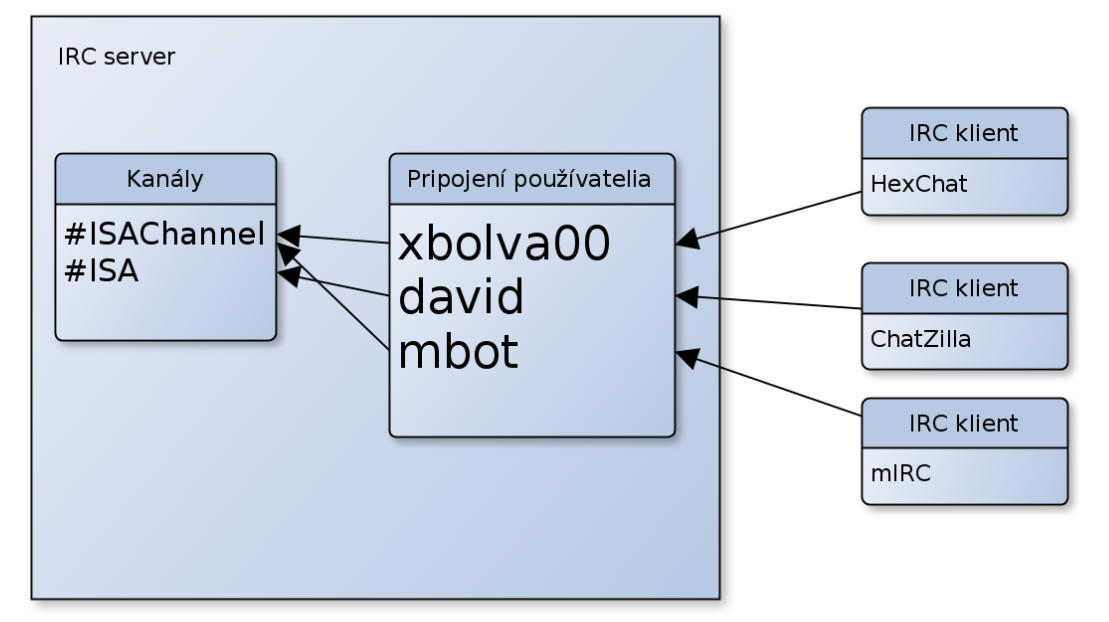
\includegraphics[width=\textwidth]{irc_arch}
	\caption{IRC klient server architektúra}
\end{figure}

\newpage

Existujú rôzne typy používateľov IRC. Zakladateľ kanálu je používateľ, ktorý založil kanál. Na danom kanáli ma najvyššie práva a kompletnú správu kanálu. Operátor kanálu má čiastočné práva na správu kanálu získané od zakladateľa kanálu. Ostatní používatelia nemajú žiadne práva na akúkoľvek správu kanálu.

Kanály sú pomenované skupiny jedného alebo viac klientov. Všetci v~tejto skupine prijímajú správy pre tento kanál. Kanál sa zakladá po pripojení prvého používateľa a zaniká po odchode posledného. Názvy kanálov začínajú znakmi @ alebo \&, nesmú obsahovať znaky medzery a čiarky a ich maximálna dĺžka je 200 znakov.

\subsection{IRC správy}
Servery a klienti si odosielajú správy medzi sebou. Ak správa obsahuje platný príkaz, klient očakáva odpoveď. Každá IRC správa obsahuje tri hlavné časti. Prvou je voliteľný \textbf{prefix}, druhou je \textbf{príkaz} a tretia časť obsahuje \textbf{parametre príkazu}. Časti su oddelené jednou alebo viacerými medzerami. Správy sú zakončené pomocou sekvencie znakov \textbf{CLRF} (\uv{\textbackslash{r}\textbackslash{n}}). V~sekcii 2.3.1 v~RFC 1459 \cite{rfc1459} je uvedený formát správy v~BNF. IRC správa nesmie presiahnuť dĺžku 512 znakov (vrátane CLRF).

\newpage

\subsection{IRC príkazy}

Významné IRC príkazy sú:
\begin{itemize}
	\item \textbf{PRIVMSG} <msgtarget> <message>
	\begin{framed}
		odoslanie správy (<message>) na cieľ (<msgtarget>) (používateľ alebo kanál).
	\end{framed}

	\item \textbf{NOTICE} <msgtarget> <message>
	\begin{framed}
		odoslanie správy (<message>) na cieľ (<msgtarget>) (používateľ alebo kanál)
		
		automatické odpovede nesmú byť odosielané ako odpovede na NOTICE správy
	\end{framed}

	\item \textbf{JOIN} <channels> [<keys>]
	\begin{framed} 
		pripojenie ku kanálom (<channels>)
	\end{framed}
	
	\item \textbf{PART} <channels> [<message>] 
	\begin{framed} 
		odchod z~kanálov <channels>
	\end{framed}
	
	\item \textbf{KICK} <channel> <client> [<message>]
	\begin{framed} 
		odstránenie klienta (<client>) z~kanálu (<channel>)
	\end{framed}

	\item \textbf{NICK} <nickname> [<hopcount>]
	\begin{framed} 
		zmena prezývky klienta
	\end{framed}

\newpage
	
	\item \textbf{PING} <server1> [<server2>] 
	\begin{framed} 
		testovanie pripojenia k~serveru
	\end{framed}
	
	\item \textbf{PONG} <server1> [<server2>] 
	\begin{framed} 
		odpoveď na PING príkaz
	\end{framed}
	
	\item \textbf{QUIT} [<message>] 
	\begin{framed} 
		odpojenie klienta od servera
	\end{framed}
\end{itemize}

\section{SYSLOG}
\textbf{Syslog} je protokol slúžiaci na zaznamenávanie správ. Protokol je opísaný v~dokumente \textbf{RFC 3164} \cite{rfc3164}. Typ architektúry je klient--server. Syslog správy je možné posielať cez \textbf{UDP aj TCP} protokoly. UDP port pridelený Syslogu je \textbf{514}, u~TCP je to \textbf{6514}. Správy sa odkazujú na zariadenia (\textbf{Facility}), ako napr. auth, deamon, local0, atď. Správam sú tiež pridelené úrovne závažnosti (\textbf{Severity})-- Emergency, Alert, Critical, Informational, atď.

\subsection{Syslog správy}
Celý formát Syslog správy sa skladá z~troch častí - \textbf{PRI}, \textbf{HEADER} a \textbf{MSG}. Celková dĺžka paketu nesmie presiahnuť 1024 bytov. \textbf{PRI} časť sa skladá z~3 až 5 znakov. Začína znakom \uv{<}, nasledovaným číslom a znakom \uv{>}. Číslo udáva prioritu, ktorá reprezentuje zariadenie/subsystém a mieru závažnosti. Túto hodnotu získame nasledovne:
\begin{framed} 
PRI = Facility * 8 + Severity
\end{framed}
Druhá časť, \textbf{HEADER}, obsahuje položku \textbf{TIMESTAMP}, kde sa nachádza dátum, čas, názov hostiteľa. Položky su oddelené medzerou. Dátum a čas je uvedený vo formáte \uv{\textbf{Mmm dd hh:mm:ss}}, kde Mmm je skrátený anglický názov mesiaca (Jan, Feb, atď.). Nasleduje \textbf{HOSTNAME} -- ak je adresa hostiteľa neznáma, použije sa IP adresa odosielateľa. Nasleduje tretia časť zvaná \textbf{MSG}, ktorá siaha až do konca paketu. Na začiatku nájdeme \textbf{TAG}, t.j. informácia o~procese/programe, ktorý správu odoslal na Syslog server. Maximálna dĺžka tohto identifikátora je 32 znakov. Prvý nealfanumerický znak značí koniec identifikátora a začiatok druhej časti, tzv. \textbf{CONTENT}, ktorý obsahuje text správy.

\begin{framed}
<PRI>TIMESTAMP HOSTNAME TAG CONTENT
\end{framed}
	
\chapter{Návrh programu}

Nasledujúci obrázok popisuje návrh samotného programu, jeho jednotlivé časti/moduly.

\begin{figure}[h]
	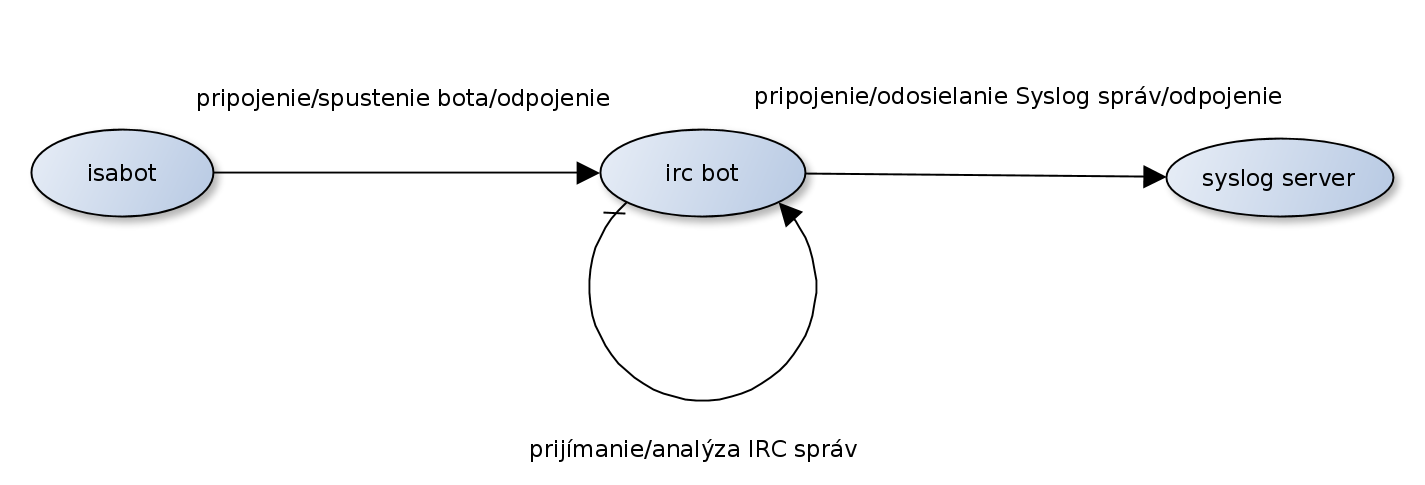
\includegraphics[width=\textwidth]{navrh}
	\caption{Návrh programu}
\end{figure}

Vstupný bod program je isabot, ktorý spracuje a skontroluje argumenty z~terminálu. Ak nedôjde k~chybe v~tejto fáze, isabot požiada IRC bota o~pripojenie k~IRC serveru na daný kanál/kanály. Následne sa spustí samotné prijímanie správ a ich analýza. IRC bot sa pripojí na Syslog server, kde sa budú zaznamenávať IRC správy, ktoré obsahujú zadané kľúčové slová. V~prípade špecifického textu v~správe spúšťa IRC bot svoje dve funkcie pre výpis dátumu alebo odoslanie správy. Po prijatí SIGINT signálu isabot požiada IRC bota o~odpojenie od IRC aj Syslog servera a program sa ukončí.

\chapter{Implementácia programu}

Program je napísaný v~jazyku C++, v~štandarde \textbf{C++14}. Sieťová komunikácia je implementovaná pomocou \textbf{BSD} schránok. Program podporuje \textbf{IPv4} aj \textbf{IPv6} adresy. IPv6 adresa musí byť zadaná spolu s portom, keďže oddelovač adresy a portu je znak dvojbodky a nebolo by možné pre program zistiť, či dvojbodka je súčasť adresy, alebo je oddelovačom adresy od portu. Jednotlivé logické celky su umiestnené v~triedach. 

V~súbore isabot.cc je samotný vstup programu (funkcia main). V~nej sa volá funkcia \textbf{parse\_args}, ktorá spracováva vstup z~terminálu. V~prípade chyby je vyhodená výnimka \textbf{argument\_exception} s~popisom chyby, ktorý sa vypíše na štandardný chybový výstup a program sa ukončí s~návratovým kódom 1. Následne sa nastavuje vlastná reakcia na prijatie SIGINT signálu -- po prijatí tohto signálu IRC bot sa odpojí od IRC servera a program sa ukončí. Ak sa nastavenie vlastnej reakcie na signál SIGINT nepodarí, program sa ukončí s~návratovým kódom 3. IRC bot sa pripája k~IRC serveru a spúšťa svoj beh. V~prípade chyby v~sieťovej komunikácii (napr. nepodarí sa pripojiť k~IRC serveru) je vyhodená výnimka \textbf{network\_exception} s~popisom chyby, ktorý sa vypíše na štandardný chybový výstup a program sa ukončí s~návratovým kódom 2. Ak nedôjde k~žiadnym chybám počas behu programu, program sa ukončí s~návratovým kódom 0 po prijatí SIGINT signálu.

Súbor irc\_bot.cc obsahuje triedu \textbf{irc\_bot}, ktorá zapuzdruje kód súvisiaci s~IRC botom. Nachádzajú sa tu funkcie pre pripojenie/odpojenie sa k~IRC serveru, spustenie samotného behu IRC bota, kde sa prijímajú a analyzujú IRC správy.

Program načítava znaku po znaku pomocou funkcie recv z~IRC servera a pripája znaky do reťazca. Po prijatí znaku sa následne kontroluje, či tento reťazec je zakončený sekvenciou znakov CLRF. Ak áno, vytvorí sa objekt triedy \textbf{irc\_command} (implementovaná v~irc\_command.cc), ktorá ponúka metódy na zistenie typu príkazu a analýzu a detekciu častí IRC správ.

Pripojenie, odosielanie správ a odpojenie od Syslog servera je implementované v~triede \textbf{syslog\_server}, implementované v~súbore syslog\_server.cc. Ďalej je tu metóda na získanie časového razítka (timestamp), ktoré je súčasťou Syslog správy. Poslednou metódou v~tejto triede je funkcia na získanie IP adresy odosielateľa, ktorá je taktiež súčasť Syslog správy.

Pomocné funkcie, ktoré sa používajú v~rôznych miestach programu, sú implementované v~súbore utils.cc. Je tu funkcia na prevod reťazca na pole (vektor) slov, slová sú v~reťazci oddelené medzerami. Ďalej je tu funkcia na prevod pola (vektoru) reťazcov na jeden reťazec, medzi jednotlivé reťazce je pridaný znak čiarky. 

\newpage

\subsection{Pripojenie ku IRC kanálu}
Po pripojení k~IRC serveru sa odošle nasledovná sekvencia IRC príkazov. Každý príkaz je zakončený sekvenciou znakov CLRF.
\begin{framed}
	NICK xbolva00
	
	USER xbolva00 xbolva00 xbolva00 :xbolva00
	
	JOIN kanál{, kanál}
\end{framed}

Ak dôjde k~chybe počas tejto fázy (ban na IRC kanáli, kanál je neplatný, atď), program sa ukončí a o~vyskytnutej chybe je používateľ informovaný správou na štandardný chybový výstup.

\newpage

\subsection{Analýza IRC správ}

Nasledujúci algoritmus popisuje implementáciu analýzy IRC správ po jej prijatí z~IRC servera.


\SetKwInput{KwData}{Vstup}
\SetKwInput{KwResult}{Výstup}

\begin{algorithm}
	\KwData{IRC správa zakončená CLRF}
	\KwResult{Spracovaná IRC správa}
	\If{príkaz PING}{
		pošli príkaz PONG s~parametrom označujúcim server z~PING správy
	} 
	\If{príkaz PRIVSMG alebo NOTICE}{
		zisti prezývku, kanál, text správy
		
		\If{kľúčové slovo sa nachádza v~slovách textu správy}{
			vytvor a odošli správu na Syslog server
		}
	
		\If{príkaz PRIVSMG a správa obsahuje kanál}{
			\If{text správy je \uv{?today}}{
				pošli príkaz PRIVMSG na IRC server, text správy je aktuálny dátum na zariadení kde beží IRC bot vo formáte \uv{dd.mm.yyyy}
			}
		
			\If{text správy je vo formáte \uv{?msg prezývka:správa}}{
				\eIf{je používateľ s~danou prezývkou pripojený na kanáli}{
					pošli príkaz PRIVMSG na IRC server, text správy je vo formáte \uv{prezývka:správa}
				} {
				    ulož si správu do interného pola (vektora) správ na neskoršie odoslanie v~prípade, že sa daný používateľ pripojený na kanál
				}
			}
		}
	}

	\If{príkaz JOIN}{
		zisti prezývku, kanál, text správy
		
		zmen stav používateľa v~interných záznamoch na stav pripojený
		
		ak existujú čakajúce správy pre tohto používateľa, odošli ich
	} 

	
	\caption{Algoritmus analýzy IRC správ}

\end{algorithm}

\newpage

\begin{algorithm}
	\KwData{IRC správa zakončená CLRF}
	\KwResult{Spracovaná IRC správa}
	\If{príkaz QUIT}{
		zisti prezývku, v~interný štruktúrach pre každý kanál nájdi tohto používateľa a zmeň jeho stav na nepripojený
	} 
	
	\If{príkaz PART}{
		zisti prezývku, kanál
		
		v~interný štruktúrach pre daný kanál/kanáli nájdi tohto používateľa a zmeň jeho stav na nepripojený
	} 

	\If{príkaz KICK}{
		zisti prezývku vyhodeného používateľa, kanál
		
		\eIf{prezývka sa zhoduje s~\uv{xbolva00}}{
			vypíš informáciu o~vyhodení IRC bota z~kanálu, ukonči program
		} {
			v~interných štruktúrach pre daný kanál/kanáli nájdi tohto používateľa a zmeň jeho stav na nepripojený
		}
	}

	\If{príkaz NICK}{
		zisti starú a novú prezývku
		
		v~interných štruktúrach zmeň starú prezývku používateľa na novú
		
		ak existujú čakajúce správy pre novú prezývku používateľa, odošli ich
	} 

	\If{príkaz RPL\_NAMREPLY (353)}{
		zisti zoznam prezývok aktuálne pripojených používateľov, kanál
		
		v~interných štruktúrach pre daný kanál nájdi týchto používateľov a zmeň ich stav na pripojený
	}
	
	\If{chyba obmedzujúca beh IRC bota}{
		zisti text správy informujúci o~chybe
		
		vypíš text o~chybe, ukonči program
	}

	\caption{Algoritmus analýzy IRC správ - pokračovanie}
		
\end{algorithm}

\newpage 

Chyby obmedzujúca beh IRC bota sú napríklad:
\begin{itemize}
	\item vyhodenie z~kanála (KICK)
	\item neplatný kanál -- ERR\_NOSUCHCHANNEL (403)
	\item pripojenie na príliš veľa kanálov -- ERR\_TOOMANYCHANNELS (403)
	\item nemožnosť odosielania správ na kanál -- ERR\_CANNOTSENDTOCHAN (404)
	\item pripojenie sa na príliš veľa kanálov -- ERR\_TOOMANYCHANNELS (405)
	\item prezývku IRC bota (\uv{xbolva00}) už niekto používa na danom kanáli -- ERR\_NICKNAMEINUSE (433)
	\item kanál je plný -- ERR\_CHANNELISFULL (471)
	\item kanál len na pozvanie -- ERR\_INVITEONLYCHAN (473)
	\item ban na kanáli -- ERR\_BANNEDFROMCHAN (474)
\end{itemize}


\subsection{Funkcie IRC bota}
Ak sa v~texte správy s~príkazom \textbf{PRIVMSG} nachádza text \uv{\textbf{?today}}, IRC bot odošle aktuálny čas vo formáte \uv{\textbf{dd.mm.yyyy}} na daný kanál získaný pomocou funkcie std::localtime. Ďalej, ak text správy sa zhoduje s~formátom \uv{\textbf{?msg prezývka:správa}}, program zistí, či používateľ s~touto prezývkou je pripojený na danom kanáli. Ak áno, pošle mu správu na daný kanál. Ak nie, správu si uloží do asociatívneho kontajnera std::map\footnote{\url{http://en.cppreference.com/w/cpp/container/map}}, kde kľúčom je reťazec (std::string\footnote{\url{http://en.cppreference.com/w/cpp/string/basic_string}}) označujúci prezývku používateľa a hodnotou je vektor reťazcov (std::vector<std::string>\footnote{\url{http://en.cppreference.com/w/cpp/container/vector}}), ktoré reprezentujú jednotlivé čakajúce správy na odoslanie. Ďalej existuje nadradený asociatívny kontajner, kde kľúčom je názov kanála a hodnotou je vyššie spomínané asociatívny kontajner s~používateľmi (na danom kanáli) a čakajúcimi správami na odoslanie pre týchto používateľov. Následne sa čaká, kým sa daný používateľ znova pripojí na kanál. Pri porovnávaní prezývok nezáleží na veľkosti písmen. Sledovanie pripojených používateľov prebieha nasledovne: po pripojení IRC bota mu IRC server zašle správu \textbf{RPL\_NAMREPLY} (353) so zoznamom aktívnych používateľov na danom kanáli a pomocou tohto zoznamu si bot zostaví prvotný zoznam používateľov a nastaví ich stav na pripojený. Následne IRC bot sleduje príkaz \textbf{JOIN}, po pripojení používateľa sa záznam pridá do tohto zoznamu so stavom používateľa ako pripojený. IRC bot sleduje príkazy \textbf{KICK}, \textbf{PART}, \textbf{QUIT}. Pri príkaze KICK sa získa prezývka vyhodeného používateľa, ak je to prezývka IRC bota (\uv{xbolva00}), program sa ukončí, lebo došlo k~obmedzeniu jeho funkcionality na danom kanáli. V~ostatných prípadoch sa v~zozname používateľov nájde daný používateľ s~touto prezývkou a jeho stav sa zmení na nepripojený. V~prípade príkazu PART si v~zozname používateľov u~kanálu, z~ktorého používateľ odišiel, nájdeme tohto používateľa a taktiež zmeníme jeho stav na nepripojený. U~príkazu QUIT sa zmení stav používateľa na nepripojený v~zozname používateľov pre každý sledovaný kanál. IRC bot sleduje aj zmenu prezývok na kanáli pomocou príkazu \textbf{NICK}, ak dôjde k~zmene, táto zmena je aplikovaná aj v~zoznamoch používateľov, ktoré si spravuje IRC bot. V~prípade, že má IRC bot uložené nejaké správy pre novú prezývku používateľa, odošle mu ich na kanál.


\subsection{Odosielanie Syslog správ}
V~prípade, že nie je zadané kľúčového slovo, IRC bot sa k~Syslog serveru nepripája, keďže nie je čo zaznamenávať. Ak je zadané jedno alebo viacero kľúčových slov oddelených čiarkou, postupuje sa nasledovne: ak sa kľúčové slovo nachádza v~IRC správe, táto správa sa odošle na Syslog server, ktorý je definovaný prepínačom -s, inak sa použije adresa localhostu, t.j. \uv{127.0.0.1}. Požiadavky v~zadaní hovoria o~tom, že zariadenie (Facility) má byť local0 (hodnota 16), a miera závažnosti nech je Informational (hodnota 6). V~kapitole 2.2.1 je uvedený vzorec na výpočet hodnoty priority Syslog správy a v~našom konkrétnom prípade je to: 16 * 8 + 6 = 134. PRI časť začína znakom \uv{<}, nasledovaný číslom priority (v~našom prípade \textbf{PRI = 134}) a znakom \uv{>}. Na získanie dátumu a času sa používa funkcia \textbf{std::localtime}, získanú štruktúru s~informáciami následne naformátujeme na formát dátumu a času, ktorý je spomenutý v~kapitole 2.2.1. IP adresu odosielateľa zisťujeme pomocou funkcie get\_ip\_address z~triedy syslog\_server, ktorá bola popísaná vyššie. Získaný časový údaj a IP adresa  odosielateľa sa uvedie do HEADER časti. Ako identifikátor procesu v~MSG časti správy sa použije názov nášho programu, t.j. \uv{isabot}. Nasleduje prezývka používateľa, ktorý danú IRC správu, ktorá sa zaznamenáva, napísal. Ďalším znakom je \uv{:}, za ktorým je samotný text správy (\textbf{CONTENT}). Takto naformátovaná správa skladajúca sa z~\textbf{PRI}, \textbf{HEADER} a \textbf{MSG} častí sa odošle Syslog server.

\subsection{Odpojenie od IRC/Syslog servera}
Po prijatí SIGINT signálu IRC bot sa odpojí od IRC servera pomocou príkazu QUIT a uzavrie pripojenie k~IRC/Syslog serveru.

\chapter{Ladenie a testovanie programu}
Spoločne s~programom za na účely testovania a ladenia používal IRC klient \textbf{HexChat} a voľne dostupný IRC bot napísaný v~Pythone, ktorý vypisoval na štandardný výstup prijaté správy od IRC servera. Tieto informácie poslúžili na overenie správnosti formátov správ, či už u~IRC alebo Syslog správ. Na ladenie chýb v~kóde sa využívali pomocné výpisy, prípadne krokovanie cez nástroj gdb. Po pripojení nášho programu, HexChatu a Python IRC bota nasledovali testy funkcií bota, kde som v~HexChate zadal, či už \uv{?today} alebo \uv{?msg prezývka:správa} a sledoval reakcie programu. Pre overenie reakcie bota na ban či vyhodenie, som sa s~touto trojicou programov pripojil na kanál, na ktorom nikto nebol, a teda som sa tam stal správcom kanálu, čo znamenalo zisk najvyšších práv na správu kanálu. V~HexChate som udelil ban/vyhodil bota z~kanála, t.j. používateľa s~prezývkou \uv{xbolva00} a sledoval ako sa program zachová, či sa správne ukončí, a pod. Testovanie Syslog správ prebiehalo tak, že som spustil Wireshark a odchytával som pakety na Loopbacku. Následne napísal nejaký text správy v~HexChate, ktorý obsahoval nejaké z~kľúčových slov a sledoval záznamy vo \textbf{Wireshark}u protokol Syslog. Záznamy som skontroloval na správnosť formátu a údajov v~nich.

\begin{figure}[h]
	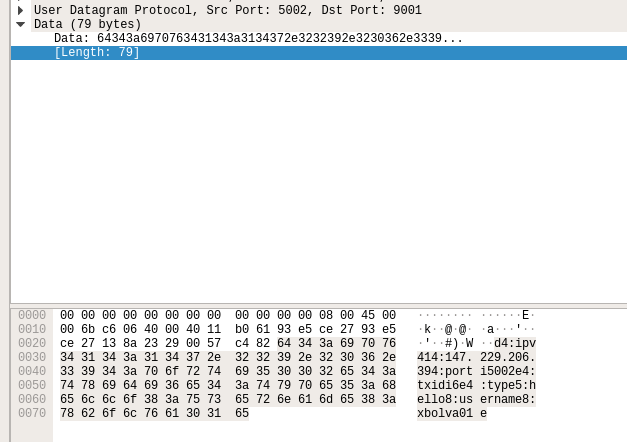
\includegraphics[width=\textwidth]{wireshark}
	\caption{Sledovanie Syslog správ vo Wiresharku}
\end{figure}


\chapter{Návod na použitie}

Program sa spúšťa cez terminál. Pri zadaní prepínača \textbf{-h/-{}-help} sa vypíše informačný text o~programe a jeho prepínačoch. V~prípade neznámeho či chybne použitého prepínača (nesprávna/chýbajúca hodnota prepínača) alebo pri akejkoľvek chybe v~sieťovej komunikácii sa program ukončí a o~probléme informuje používateľa správou na štandardný chybový výstup.

\begin{framed}
Použitie: isabot HOST[:PORT] CHANNELS [-s SYSLOG\_SERVER] [-l HIGHLIGHT] [-h|--help]

HOST je názov/IP adresa servera (napr. irc.freenode.net)

PORT je číslo portu (predvolené je 6667)

CHANNELS obsahuje jeden alebo viac kanálov (začínajú znakom \# alebo \&, oddelené sú čiarkou)

-s SYSLOG\_SERVER je IP adresa Syslog servera

-l HIGHLIGHT je zoznam kľúčových slov oddelených čiarkou (napr. ip,tcp,udp,isa)

-h|-{}-help zobrazenie informácii o~programe a o~prepínačoch
\end{framed}

Program sa ukončuje pomocou \textbf{Ctrl-C}, resp. pomocou príkazu \uv{\textbf{kill -INT <pid>}} v~termináli.


\chapter{Informácie o~programe}

Program sa skladá z~Makefile, ktorý slúži na zostavenie programu a nasledovných zdrojových súborov:

\begin{itemize}
\item isabot.cc
\item isabot.h
\item irc\_bot.cc
\item irc\_bot.h
\item irc\_command.cc
\item irc\_command.h
\item syslog\_server.cc
\item syslog\_server.h
\item utils.cc
\item utils.h
\end{itemize}

Spolu sa jedná o~813 riadkov zdrojového textu. Veľkosť výsledného binárneho súboru je 91,2 kB (preložené s~-02).

\chapter{Záver}
Projekt mal za cieľ vyskúšať si programovanie sieťovej služby. Bolo potrebné si naštudovať IRC a Syslog protokoly z~RFC dokumentov a následne tieto získané znalosti aplikovať v~implementácii samotného programu. Projekt overil nielen komplexne znalosti (analýza RFC dokumentov, práca s~BSD schránkami, programovanie v~C++, atď.) ale aj programatorské zručnosti - návrh, implementácia, ladenie a testovanie programu. Novozískané vedomosti z~tohto projektu sa týkali hlavne programovania sieťových aplikácií a protokolov (IRC, Syslog), na čo sú, čo umožňujú a ako fungujú.
 % viz. obsah.tex / see obsah.tex

  % Pouzita literatura / Bibliography
  % ----------------------------------------------
\ifslovak
  \makeatletter
  \def\@openbib@code{\addcontentsline{toc}{chapter}{Literatúra}}
  \makeatother
  \bibliographystyle{bib-styles/czechiso}
\else
  \ifczech
    \makeatletter
    \def\@openbib@code{\addcontentsline{toc}{chapter}{Literatura}}
    \makeatother
    \bibliographystyle{bib-styles/czechiso}
  \else 
    \makeatletter
    \def\@openbib@code{\addcontentsline{toc}{chapter}{Bibliography}}
    \makeatother
    \bibliographystyle{bib-styles/englishiso}
  %  \bibliographystyle{alpha}
  \fi
\fi
  \begin{flushleft}
  \bibliography{projekt-20-literatura-bibliography}
  \end{flushleft}

  % vynechani stranky v oboustrannem rezimu
  % Skip the page in the two-sided mode
  \iftwoside
    \cleardoublepage
  \fi

  % Prilohy / Appendices
  % ---------------------------------------------
  \appendix
\ifczech
  \renewcommand{\appendixpagename}{Přílohy}
  \renewcommand{\appendixtocname}{Přílohy}
  \renewcommand{\appendixname}{Příloha}
\fi
\ifslovak
  \renewcommand{\appendixpagename}{Prílohy}
  \renewcommand{\appendixtocname}{Prílohy}
  \renewcommand{\appendixname}{Príloha}
\fi

% vynechani stranky v oboustrannem rezimu
% Skip the page in the two-sided mode
\iftwoside
  \cleardoublepage
\fi
  
\ifslovak
%  \section*{Zoznam príloh}
%  \addcontentsline{toc}{section}{Zoznam príloh}
\else
  \ifczech
%    \section*{Seznam příloh}
%    \addcontentsline{toc}{section}{Seznam příloh}
  \else
%    \section*{List of Appendices}
%    \addcontentsline{toc}{section}{List of Appendices}
  \fi
\fi
  \startcontents[chapters]
  % seznam příloh / list of appendices
  % \printcontents[chapters]{l}{0}{\setcounter{tocdepth}{2}}
  
  % vynechani stranky v oboustrannem rezimu
  \iftwoside
    \cleardoublepage
  \fi
  % % Tento soubor nahraďte vlastním souborem s přílohami (nadpisy níže jsou pouze pro příklad)
% This file should be replaced with your file with an appendices (headings below are examples only)

% Umístění obsahu paměťového média do příloh je vhodné konzultovat s vedoucím
% Placing of table of contents of the memory media here should be consulted with a supervisor
%\chapter{Obsah přiloženého paměťového média}

%\chapter{Manuál}

%\chapter{Konfigurační soubor} % Configuration file

%\chapter{RelaxNG Schéma konfiguračního souboru} % Scheme of RelaxNG configuration file

%\chapter{Plakát} % poster

\chapter{Jak pracovat s touto šablonou}
\label{jak}

V této kapitole je uveden popis jednotlivých částí šablony, po kterém následuje stručný návod, jak s touto šablonou pracovat. 

Jedná se o přechodnou verzi šablony. Nová verze bude zveřejněna do konce roku 2016 a bude navíc obsahovat nové pokyny ke správnému využití šablony, závazné pokyny k~vypracování bakalářských a diplomových prací (rekapitulace pokynů, které jsou dostupné na~webu) a nezávazná doporučení od vybraných vedoucích. Jediné soubory, které se v nové verzi změní, budou projekt-01-kapitoly-chapters.tex a projekt-30-prilohy-appendices.tex, jejichž obsah každý student vymaže a nahradí vlastním. Šablonu lze tedy bez problémů využít i~v~současné verzi.

\section*{Popis částí šablony}

Po rozbalení šablony naleznete následující soubory a adresáře:
\begin{DESCRIPTION}
  \item [bib-styles] Styly literatury (viz níže). 
  \item [obrazky-figures] Adresář pro Vaše obrázky. Nyní obsahuje placeholder.pdf (tzv. TODO obrázek, který lze použít jako pomůcku při tvorbě technické zprávy), který se s prací neodevzdává. Název adresáře je vhodné zkrátit, aby byl jen ve zvoleném jazyce.
  \item [template-fig] Obrázky šablony (znak VUT).
  \item [fitthesis.cls] Šablona (definice vzhledu).
  \item [Makefile] Makefile pro překlad, počítání normostran, sbalení apod. (viz níže).
  \item [projekt-01-kapitoly-chapters.tex] Soubor pro Váš text (obsah nahraďte).
  \item [projekt-20-literatura-bibliography.bib] Seznam literatury (viz níže).
  \item [projekt-30-prilohy-appendices.tex] Soubor pro přílohy (obsah nahraďte).
  \item [projekt.tex] Hlavní soubor práce -- definice formálních částí.
\end{DESCRIPTION}

Výchozí styl literatury (czechiso) je od Ing. Martínka, přičemž anglická verze (englishiso) je jeho překladem s drobnými modifikacemi. Oproti normě jsou v něm určité odlišnosti, ale na FIT je dlouhodobě akceptován. Alternativně můžete využít styl od Ing. Radima Loskota nebo od Ing. Radka Pyšného\footnote{BP Ing. Radka Pyšného \url{http://www.fit.vutbr.cz/study/DP/BP.php?id=7848}}. Alternativní styly obsahují určitá vylepšení, ale zatím nebyly řádně otestovány větším množstvím uživatelů. Lze je považovat za beta verze pro zájemce, kteří svoji práci chtějí mít dokonalou do detailů a neváhají si nastudovat detaily správného formátování citací, aby si mohli ověřit, že je vysázený výsledek v pořádku.

Makefile kromě překladu do PDF nabízí i další funkce:
\begin{itemize}
  \item přejmenování souborů (viz níže),
  \item počítání normostran,
  \item spuštění vlny pro doplnění nezlomitelných mezer,
  \item sbalení výsledku pro odeslání vedoucímu ke kontrole (zkontrolujte, zda sbalí všechny Vámi přidané soubory, a případně doplňte).
\end{itemize}

Nezapomeňte, že vlna neřeší všechny nezlomitelné mezery. Vždy je třeba manuální kontrola, zda na konci řádku nezůstalo něco nevhodného -- viz Internetová jazyková příručka\footnote{Internetová jazyková příručka \url{http://prirucka.ujc.cas.cz/?id=880}}.

\paragraph {Pozor na číslování stránek!} Pokud má obsah 2 strany a na 2. jsou jen \uv{Přílohy} a~\uv{Seznam příloh} (ale žádná příloha tam není), z nějakého důvodu se posune číslování stránek o 1 (obsah \uv{nesedí}). Stejný efekt má, když je na 2. či 3. stránce obsahu jen \uv{Literatura} a~je možné, že tohoto problému lze dosáhnout i jinak. Řešení je několik (od~úpravy obsahu, přes nastavení počítadla až po sofistikovanější metody). \textbf{Před odevzdáním proto vždy překontrolujte číslování stran!}


\section*{Doporučený postup práce se šablonou}

\begin{enumerate}
  \item \textbf{Zkontrolujte, zda máte aktuální verzi šablony.} Máte-li šablonu z předchozího roku, na stránkách fakulty již může být novější verze šablony s~aktualizovanými informacemi, opravenými chybami apod.
  \item \textbf{Zvolte si jazyk}, ve kterém budete psát svoji technickou zprávu (česky, slovensky nebo anglicky) a svoji volbu konzultujte s vedoucím práce (nebyla-li dohodnuta předem). Pokud Vámi zvoleným jazykem technické zprávy není čeština, nastavte příslušný parametr šablony v souboru projekt.tex (např.: \verb|documentclass[english]{fitthesis}| a přeložte prohlášení a poděkování do~angličtiny či slovenštiny.
  \item \textbf{Přejmenujte soubory.} Po rozbalení je v šabloně soubor projekt.tex. Pokud jej přeložíte, vznikne PDF s technickou zprávou pojmenované projekt.pdf. Když vedoucímu více studentů pošle projekt.pdf ke kontrole, musí je pracně přejmenovávat. Proto je vždy vhodné tento soubor přejmenovat tak, aby obsahoval Váš login a (případně zkrácené) téma práce. Vyhněte se však použití mezer, diakritiky a speciálních znaků. Vhodný název tedy může být např.: \uv{xlogin00-Cisteni-a-extrakce-textu.tex}. K přejmenování můžete využít i přiložený Makefile:
\begin{verbatim}
make rename NAME=xlogin00-Cisteni-a-extrakce-textu
\end{verbatim}
  \item Vyplňte požadované položky v souboru, který byl původně pojmenován projekt.tex, tedy typ, rok (odevzdání), název práce, svoje jméno, ústav (dle zadání), tituly a~jméno vedoucího, abstrakt, klíčová slova a další formální náležitosti.
  \item Nahraďte obsah souborů s kapitolami práce, literaturou a přílohami obsahem svojí technické zprávy. Jednotlivé přílohy či kapitoly práce může být výhodné uložit do~samostatných souborů -- rozhodnete-li se pro toto řešení, je doporučeno zachovat konvenci pro názvy souborů, přičemž za číslem bude následovat název kapitoly. 
  \item Nepotřebujete-li přílohy, zakomentujte příslušnou část v projekt.tex a příslušný soubor vyprázdněte či smažte. Nesnažte se prosím vymyslet nějakou neúčelnou přílohu jen proto, aby daný soubor bylo čím naplnit. Vhodnou přílohou může být obsah přiloženého paměťového média.
  \item Nascanované zadání uložte do souboru zadani.pdf a povolte jeho vložení do práce parametrem šablony v projekt.tex (\verb|documentclass[zadani]{fitthesis}|).
  \item Nechcete-li odkazy tisknout barevně (tedy červený obsah -- bez konzultace s vedoucím nedoporučuji), budete pro tisk vytvářet druhé PDF s tím, že nastavíte parametr šablony pro tisk: (\verb|documentclass[zadani,print]{fitthesis}|).  Barevné logo se nesmí tisknout černobíle!
  \item Vzor desek, do kterých bude práce vyvázána, si vygenerujte v informačním systému fakulty u zadání. Pro disertační práci lze zapnout parametrem v šabloně (více naleznete v souboru fitthesis.cls).
  \item Nezapomeňte, že zdrojové soubory i (obě verze) PDF musíte odevzdat na CD či jiném médiu přiloženém k technické zprávě.
\end{enumerate}

\subsection*{Pokyny pro oboustranný tisk}
\begin{itemize}
\item Zapíná se parametrem šablony: \verb|\documentclass[twoside]{fitthesis}|
\item Po vytištění oboustranného listu zkontrolujte, zda je při prosvícení sazební obrazec na obou stranách na stejné pozici. Méně kvalitní tiskárny s duplexní jednotkou mají často posun o 1--3 mm. Toto může být u některých tiskáren řešitelné tak, že vytisknete nejprve liché stránky, pak je dáte do stejného zásobníku a vytisknete sudé.
\item Za titulním listem, obsahem, literaturou, úvodním listem příloh, seznamem příloh a případnými dalšími seznamy je třeba nechat volnou stránku, aby následující část začínala na liché stránce (\textbackslash cleardoublepage).
\item  Konečný výsledek je nutné pečlivě překontrolovat.
\end{itemize}


\subsection*{Užitečné nástroje}
\label{nastroje}

Následující seznam není výčtem všech využitelných nástrojů. Máte-li vyzkoušený osvědčený nástroj, neváhejte jej využít. Pokud však nevíte, který nástroj si zvolit, můžete zvážit některý z následujících:

\begin{description}
	\item[\href{http://miktex.org/download}{MikTeX}] \LaTeX{} pro Windows -- distribuce s jednoduchou instalací a vynikající automatizací stahování balíčků.
	\item[\href{http://texstudio.sourceforge.net/}{TeXstudio}] Přenositelné opensource GUI pro \LaTeX{}.  Ctrl+klik umožňuje přepínat mezi zdrojovým textem a PDF. Má integrovanou kontrolu pravopisu, zvýraznění syntaxe apod. Pro jeho využití je nejprve potřeba nainstalovat MikTeX.
	\item[\href{http://jabref.sourceforge.net/download.php}{JabRef}] Pěkný a jednoduchý program v Javě pro správu souborů s bibliografií (literaturou). Není potřeba se nic učit -- poskytuje jednoduché okno a formulář pro editaci položek.
	\item[\href{https://inkscape.org/en/download/}{InkScape}] Přenositelný opensource editor vektorové grafiky (SVG i PDF). Vynikající nástroj pro tvorbu obrázků do odborného textu. Jeho ovládnutí je obtížnější, ale výsledky stojí za to.
	\item[\href{https://git-scm.com/}{GIT}] Vynikající pro týmovou spolupráci na projektech, ale může výrazně pomoci i jednomu autorovi. Umožňuje jednoduché verzování, zálohování a přenášení mezi více počítači.
	\item[\href{http://www.overleaf.com/}{Overleaf}] Online nástroj pro \LaTeX{}. Přímo zobrazuje náhled a umožňuje jednoduchou spolupráci (vedoucí může průběžně sledovat psaní práce), vyhledávání ve zdrojovém textu kliknutím do PDF, kontrolu pravopisu apod. Zdarma jej však lze využít pouze s určitými omezeními (někomu stačí na disertaci, jiný na ně může narazit i při psaní bakalářské práce) a pro dlouhé texty je pomalejší.
\end{description}

\subsection*{Užitečné balíčky pro \LaTeX}

Studenti při sazbě textu často řeší stejné problémy. Některé z nich lze vyřešit následujícími balíčky pro \LaTeX:

\begin{itemize}
  \item \verb|amsmath| -- rozšířené možnosti sazby rovnic,
  \item \verb|float, afterpage, placeins| -- úprava umístění obrázků,
  \item \verb|fancyvrb, alltt| -- úpravy vlastností prostředí Verbatim, 
  \item \verb|makecell| -- rozšíření možností tabulek,
  \item \verb|pdflscape, rotating| -- natočení stránky o 90 stupňů (pro obrázek či tabulku),
  \item \verb|hyphenat| -- úpravy dělení slov,
  \item \verb|picture, epic, eepic| -- přímé kreslení obrázků.
\end{itemize}

Některé balíčky jsou využity přímo v šabloně (v dolní části souboru fitthesis.cls). Nahlédnutí do jejich dokumentace může být rovněž užitečné.

Sloupec tabulky zarovnaný vlevo s pevnou šířkou je v šabloně definovaný \uv{L} (používá se jako \uv{p}).

 % viz. prilohy.tex / see prilohy.tex
\end{document}
